%to have line numbers
%\RequirePackage{lineno}
\documentclass[10pt, letterpaper]{article}      
\usepackage[margin=.1cm,font=small,labelfont=bf]{caption}[2007/03/09]
%\usepackage{endnotes}
%\let\footnote=\endnote
\usepackage{setspace}
\usepackage{longtable}                        
\usepackage{anysize}                          
\usepackage{natbib}                           
%\bibpunct{(}{)}{,}{a}{,}{,}                   
\bibpunct{(}{)}{,}{a}{}{,}                   
\usepackage{amsmath}
\usepackage[% draft,
pdftex]{graphicx} %draft is a way to exclude figures                
\usepackage{epstopdf}
\usepackage{hyperref}                             % For creating hyperlinks in cross references

 
% \usepackage[margins]{trackchanges}

% \note[editor]{The note}
% \annote[editor]{Text to annotate}{The note}
%    \add[editor]{Text to add}
% \remove[editor]{Text to remove}
% \change[editor]{Text to remove}{Text to add}

%TODO make it more standard before submission: \marginsize{2cm}{2cm}{1cm}{1cm}
\marginsize{1cm}{1cm}{.5cm}{.5cm}%{left}{right}{top}{bottom}   
					          % Helps LaTeX put figures where YOU want
 \renewcommand{\topfraction}{1}	                  % 90% of page top can be a float
 \renewcommand{\bottomfraction}{1}	          % 90% of page bottom can be a float
 \renewcommand{\textfraction}{0.0}	          % only 10% of page must to be text

 \usepackage{float}                               %latex will not complain to include float after float

\usepackage[table]{xcolor}                        %for table shading
\definecolor{gray90}{gray}{0.90}
\definecolor{orange}{RGB}{255,128,0}

\renewcommand\arraystretch{.9}                    %for spacing of arrays like tabular

%-------------------- my commands -----------------------------------------
\newenvironment{ig}[1]{
\begin{center}
 %\includegraphics[height=5.0in]{#1} 
 \includegraphics[height=3.3in]{#1} 
\end{center}}

 \newcommand{\cc}[1]{
\hspace{-.13in}$\bullet$\marginpar{\begin{spacing}{.6}\begin{footnotesize}\color{blue}{#1}\end{footnotesize}\end{spacing}}
\hspace{-.13in} }

%-------------------- END my commands -----------------------------------------



%-------------------- extra options -----------------------------------------

%%%%%%%%%%%%%
% footnotes %
%%%%%%%%%%%%%

%\long\def\symbolfootnote[#1]#2{\begingroup% %these can be used to make footnote  nonnumeric asterick, dagger etc
%\def\thefootnote{\fnsymbol{footnote}}\footnote[#1]{#2}\endgroup}	%see: http://help-csli.stanford.edu/tex/latex-footnotes.shtml

%%%%%%%%%%%
% spacing %
%%%%%%%%%%%

% \abovecaptionskip: space above caption
% \belowcaptionskip: space below caption
%\oddsidemargin 0cm
%\evensidemargin 0cm

%%%%%%%%%
% style %
%%%%%%%%%

%\pagestyle{myheadings}         % Option to put page headers
                               % Needed \documentclass[a4paper,twoside]{article}
%\markboth{{\small\it Politics and Life Satisfaction }}
%{{\small\it Adam Okulicz-Kozaryn\footnote{I thank \textbf{TODO}. All mistakes
%are mine.}} }

%\headsep 1.5cm
% \pagestyle{empty}			% no page numbers
% \parindent  15.mm			% indent paragraph by this much
% \parskip     2.mm			% space between paragraphs
% \mathindent 20.mm			% indent math equations by this much

%%%%%%%%%%%%%%%%%%
% extra packages %
%%%%%%%%%%%%%%%%%%

\usepackage{datetime}


\usepackage[latin1]{inputenc}
\usepackage{tikz}
\usetikzlibrary{shapes,arrows,backgrounds}


%\usepackage{color}					% For creating coloured text and background
%\usepackage{float}
\usepackage{subfig}                                     % for combined figures

\renewcommand{\ss}[1]{{\colorbox{blue}{\bf \color{white}{#1}}}}
\newcommand{\ee}[1]{\endnote{\vspace{-.10in}\begin{spacing}{1.0}{\normalsize #1}\end{spacing}\vspace{.20in}}}
\newcommand{\emd}[1]{\ExecuteMetaData[/tmp/tex]{#1}} % grab numbers  from stata

%TODO before submitting comment this out to get 'regular fornt'
\usepackage{sectsty}
\allsectionsfont{\normalfont\sffamily}
\usepackage{sectsty}
\allsectionsfont{\normalfont\sffamily}
\renewcommand\familydefault{\sfdefault}

\usepackage[margins]{trackchanges}
\usepackage{rotating}
\usepackage{catchfilebetweentags}

\usepackage{abstract}
\renewcommand{\abstractname}{}    % clear the title
\renewcommand{\absnamepos}{empty} % originally center

\usepackage{pgfplotstable}
% -------------------- END extra options -----------------------------------------
\date{{}\today  \hspace{.2in}\xxivtime}
\title{  % remember to have Vistula University!!
%  Happiness is Flextime, part 2: the opposite of flextime, unpredictability
%\textbf{out of date--aper done in goog doc :(}
%city unhappiness is universal across the deveoped world--no cant say that bc
%they are not significant
The Urban-Rural Happiness Gradient Across Countries:\\
City Unhappiness is Common \\ 
(Despite What Economists Say) %Claims to the Contrary by
}
\author{
% Adam Okulicz-Kozaryn\thanks{EMAIL: adam.okulicz.kozaryn@gmail.com
%   \hfill I thank XXX.  All mistakes are mine.} \\
% {\small Rutgers - Camden  and Vistula University}
}

\begin{document}

%%\setpagewiselinenumbers
%\modulolinenumbers[1]
%\linenumbers

\bibliographystyle{/home/aok/papers/root/tex/ecta}
\maketitle
\vspace{-.4in}
\begin{center}

\end{center}


\begin{abstract}
This study shows, for the first time, that city unhappiness is 
common across the World.
%
In no developed country, people are happier in larger places than in
smaller places.
Without exception, in no developed country city is happier than smaller areas.
%
The finding is important because there are
 economists manipulating data through cherry-picking
\citep[e.g.,][]{glaeser11,glaeser14,burger20} and claiming the opposite, that
urban areas are happier. Such manipulation is arguably for ideological
reasons. The axioms of economics are that the greater production, productivity,
income, and consumption, the better. Urban areas produce most% , are most
% productive
, and most income and consumption take place there.
Economics' concept of utility is directly linked to consumption: the more
consumption, the more utility. While utility cannot be measured, economists
appear to try to show that happiness is greatest where economics axioms point
to, in cities. Sociological, psychological, and neurological evidence is ignored
% and research having little to do with reality is produced
. Present study is
correlational, not experimental, and causality cannot be claimed. 
\end{abstract}
\vspace{.15in} 
\noindent{\sc % Happiness, Life Satisfaction,  Subjective Wellbeing  (SWB),
              % Cities, Urbaniciy, Urban-Rural, Urban-Rural Gradient, World Vaues Survey (WVS)
}
\vspace{.25in} 

We know that in many countries there is a so called  ``urban-rural happiness''
gradient \cite{aok11a}, where happiness raises from lowest in largest cities to
highest in smallest places. The gradient is non-linear, the very largest cities
are markedly less happy than all other areas in a country: New York City \citep{aok_brfss_city_cize16,
  senior_ny_sep16_14}, London \citep{ons11,ibt13} Helsinki \citep{morrison15}, Bucharest \citep{lenzi16D}, Sydney
\citep[cited in][]{morrison11}.
The goal of this paper is to test gradient across countries using one dataset
with uniform variables. This study shows, for the first time, that city unhappiness is 
 common across the World \footnote{Most extant research about the urban-rural
   happiness gradient  is about
   the US, Western Europe, recently China, and handful of
other countries. Again, there were studies conducted in
   single countries, but not using a uniform dataset across countries. The three
   apparent exceptions \citep{aokcities,burger20,easterlin10al} are not
   exceptions. No study studies the gradient, all use binary urban-rural
   operationalizations and present simple mean differences for each country and
   aggregate results to groups of countries in regressions  as elaborated later.
   %
Last but not least, Gallup data used by \citet{burger20} and
\citet{easterlin10al} are highly problematic as elaborated later.}
 
Intersection of % QOL/SWB
Quality Of Life (QOL) or Subjective Wellbeing (SWB)\footnote{The two, SWB and
  QOL overlap, but there are important differences, notably QOL is more of an
  index/aggregate of domains and more subjective, while SWB is subjective mostly
evaluation of one's life as a whole--for discussion see \citet{aok-swbLivability18}.}  and Urban Studies is an exciting area.
Academics, policymakers, administrators, and common people start to pay more
attention to QOL/SWB, not just monetary measures such as GDP. We finally begin to realize, even some economists do
\citep{stiglitz09al}, that money is not everything and it is high time to look at human
flourishing: QOL and SWB. 
%
 But some economists
manipulate data through cherry-picking \citep{glaeser11,glaeser14,burger20} and
try to claim the opposite, that cities are happier--the present study provides
yet more evidence that economists' thesis of city happiness is false.
 
The world is experiencing massive
urbanization--urbanization is arguably the most dramatic change to our way of life \cite{wirth38,hansonCityJournalautumn15}, and what arguably matters most
is human QOL/SWB. Hence, the question, how cities affect human condition? 
%meh could ut UN figures that in 1850 was like 10perc, by 2050 will be like 70perc

% TODO once RR add:
% For review of urbanicitysee \citet{aokCityBook15}. This study is an extension
% and follow-up on \citet{aokcities}. For review of the literature on urbanicity
% and happiness see \citet{aokCityBook15}.

Modern research on the effect of cities on human wellbeing should be founded on
extensive classic urban sociological research \citep{tonnies57,wirth38,simmel03,park15,park84}, 
which argued negative effect of cities on humans.
%
Quantitative research on the urban-rural happiness gradient dates back to
\citep{gurin60,campbell76etal}, who also found negative effect of
urbanicity on humans. And over past several decades, several dozen studies
mostly found negative effect of urbanicity on human wellbeing as well
\texttt{[blind for peer-review]}% --for review see \citet{aokCityBook15}
. 

Yet most research in the area is about the US, Western Europe, and recently China and handful of
other countries. Most studies are conducted in a single country. Hence, we offer
the present study using a uniform dataset across countries.

First, we briefly define SWB and mechanisms that are likely to link size of a
place to SWB. 
% would produce SWB from size of a place.
  
   
\section{SWB}

Subjective Wellbeing (SWB) is an umbrella term for various subjective measures
of wellbeing, notably positive and negative affects, happiness, and life
satisfaction. Most of the SWB research, including this study, uses life satisfaction measure, which is
a global self evaluation of one's life as a whole. This measure is mostly
cognitive and not affective--respondent evaluates her life as whole globally (everything,
including professional, personal, family, community, etc). The measure captures
everything that is going on in one's life--that's a major advantage of SWB
measure over other social and economic indicators aiming at measuring human
condition, progress, and development. SWB measure is simply the most
comprehensive measure possible dwarfing earlier measures such as income,
education, or life expectancy. For review see \citet{diener09}.
%TODO once RR add \cite{aok_lsPol16}

Following usual practice, for simplicity, we use these terms interchangeably: SWB, happiness, and
life satisfaction, but specifically we mostly mean life satisfaction as defined above.

SWB measure is also at least adequately reliable and valid and considered good
enough for public policy making and public administration
\citep{diener09,stiglitz09al}. And it has been used multiple times in urban
research \citep[e.g.,][]{moeinaddini20,mouratidis19,wang19,anon17-cities-oslo,ma17,wkeziak16,valente16,chen15}.

There are cross-cultural comparability caveats, however, and SWB may not be
adequately comparable across countries \citep{kahneman99,diener09}. This limitation should be kept in
mind when comparing results across countries in the present study. And more
focus should be on within-country differences, and this is what this study is
mostly about--the difference between smaller and larger places in terms of SWB
within countries. We treat each country separately and do not pull the data
together. In short, one should focus on within-country differences across
urbanicity and exercise caution when comparing effects across countries. 

\section{Urban Definition, Theory, and Potential Causal Mechanism/Pathway}

{This
  is an observational study, not an experiment, and we don't test causality here,
  nevertheless it is important to discuss the potential mechanisms.}

It is useful to start with the theory that would define urbanicity and predict how
% different place sizes
urbanness would affect SWB. % Defining mechanisms first helps to define urbanicity.
% In other words, we present rationality for urbanicity definition with respect to
% swb. There is a mechanism that would produce different outcomes in swb by
% urbanicity.
% % and so this is limitation of easterlin and burger
% % to economists this is perhaps urban=developed/money making, rural=backwards/not  making money.
% Note that this is rather illustratibe than exhaustive and full presentation is
% beyond the scope of this study.
%
We start with classic urban sociological theory of urban malaise
 \citep{tonnies57,wirth38,simmel03,park15,park84}: cities produce superficiality,
transitoriness, withdrawal, impersonality, superficiality, deviance,
shallowness, anomie, alienation, and cognitive overload.\footnote{Classics
  argued poor social ties in cities, but see later arguments by Fischer  and his
  subcultural theory \citep{fischer95,fischer75,fischer72}.} 
 Sociological theory is not clear at which point urban malaise arises, there is clearly no hard
cutoff point, rather, the more urban, the more malaise. There may be a certain
threshold though, at which malaise intensifies as hinted at by
\citet{fischer73}: in the largest cities% , $>$several hundred thousand
.
 In the classical urban sociology city is defined by large population size, density,
and heterogeneity \citep{wirth38}. To sum up, urbanicity has mostly negative
effect on humans, and it is rather a continuum than binary, although a threshold
at a population of several hundred thousand may exist where malaise intensifies.

Another indication of continuity in effect of size of a place on human condition
comes from physics% , and clearly points to a continuum
. There is physical city
constant of 1.15: double area's population size and many phenomena (crime, GDP, income, patents)  increase by 15\% \citep{blissCL_nov4_14,bettencourt10,bettencourt10b,bettencourt07}.

We would like to especially highlight biological/evolutionary mechanism.
%LATER/MAYBE meh for now skip the ingroup
% namely enviorment where humans evolved and related ingroup preference.
% Here too, it is continuum, not binary--the larger the place, the farther it is
% from where we eveolved and the more outgroups.
%
For over 95\% of our evolutionary history\footnote{% Already Simmel observed
   % that old cities had a character of today's small town--for instance see
   % \citet[p. 333]{simmel03}.
Per human species evolutionary history, for  instance, see encyclopedia Britannica
   \url{http://www.britannica.com/EBchecked/topic/277071/hunting-and-gathering-culture}. 
    % Wikipedia
   % \url{http://en.wikipedia.org/wiki/List_of_largest_cities_throughout_history},
   % and  also see .
   For post-medieval history see \citet{white77}.%  World population percent living in cities larger than 100k
   % is from , table 1. 
 } we have lived outside of the cities as
hunter-gatherers usually in small bands of 50-80 people \citep{maryanski92}.
 It only started to slowly change in about 10,000 BC  with domestication of animals
 and agriculture. The first large cities (larger than several hundred thousand% again,$>$250k
 ) only started to emerge
 after 500 BC and there were just handful of them. 
 It wasn't really
 until after industrialization that large cities started to house noticeable 
 proportion of the  population, and only 20th century saw urbanization explosion--in
 1800 a mere 1.7\% of the world population lived in cities larger than 100k, it
 slowly increased to 2.3\% in 1850, by another 50 years doubled to 5.5\% in 1900,
 and then it doubled again to 13\% in 1950 \citep{davis55}.

The larger the place, the more the % built
environment differs from the habitat in
which we have evolved: dense and crowded,\footnote{There are striking examples of crowding in largest cities.  To
  be sure, majority of urban population does not live in such extreme crowding,
  the trend however is in that direction as cities are becoming larger and less
  affordable. And, again, even without extreme crowding, usual population
  density is related to crime \citep{bettencourt10b}. There is also evidence
  that density relates to negative consequences: interestingly there is evidence
  that density impacts pathology more than crowding
  \citep{levy1974effects}. Yet, it is not only density and crowding, other
  factors such as social support matter as well \citep{cassel2017health}. Some
  studies didn't find negative effects of density or crowding and results were
  mixed \citep{collette1976urban}. While it seems to be reasonable to assume
  that density and crowding are positively related, some studies do not find
  this to be the case \citep{webb1975meaning,rodgers1982density}
  .
Crowding probably has become more common in recent years as cities are becoming
less affordable. \citet{misraCL15oct6,floridaCL18apr11,weinbergCL16aug11,solariMISC19apr24,schuetzMISC19may7,kotkin_db_mar20_13}
  
  For a nice discussion and overview of density, crowding and human behavior see \citet{boots1979population,choldin1978urban}.}
airport, subway or rapid transit, tall buildings in downtown, etc. And
again, while clearly urbanness is a continuum, there is likely a threshold,  around
 several hundred thousand people, when the built environment changes
 significantly.
%
 The are at least several significantly different stages of urbanness on the
 urbanness continuum. There is
 wilderness, open country, villages, small towns, large towns, cities, large
 cities, and very large cities. Surely, it is difficult to capture urbanness in
 its entirety--most dataset only allow few stages, including the data used
 here. But the point is that treating urbanness as an urban-rural dichotomy \citep[][]{glaeser11,burger20} is an
 oversimplification without much theory to support it.
% In addition to size, there is also density: eg suburbs can be large but relatively few people live there per square kilometer.
% And agglomerations and networks as per central place theory (cite) it is not only size or density of a place but also proximity to other places. Such information is however usually missing from data (also missing here in WVS).

 The biological/evolutionary perspective can be complemented by recent
 neurological evidence. Urban living is unhealthy to human brain \citep{lederbogen11} and urban
living contributes to the development of psychosis \citep{abrahamyan20}.
 
\section{The Problem With Economics} % OR COMBINE WITH NEXT ONE
% \section{the three studies on urban rural happiness gradient across countries}

There are  % many ``maverick economists'' studying ``economics of happiness.'' There
% are even few serious
 economists serious about studying happiness,
% that have truly contributed to social indicators
% literature,
 Richard Easterlin and Andrew Oswald among them.
%
 But sometimes, economists' interest in happiness is more of a hindrance
 than help.
%
%  , because biased and
% flawed research is produced.
%
% like one by stiupd wolfers too about income and happiness, that it is ot
%quadratic and just take the log lol
%

Economics is a discipline crippled by its ``axioms'' (the self evident truths)
or ``laws.'' No other social science boasts laws or axioms for a good
reason--they do not exist in social world, and so they should not appear in
social science. % And so the very foundation of economics, its axioms and laws,
See \citet{feynman81} for elaboration.
 
The bizarre economic axioms that have little to do with reality
\citep{davies18}, do arguably % sometimes unfortunatelly
% research forces data to agree with these
% axioms
bias many economic investigations--many economists appear to try hard to force
 the data to support their axioms, intentionally or unintentionally, but at the
 end, misleading and flawed research is produced. 
% 
To economists, by definition (it's the law or the axiom), the more money (income
or consumption), the greater the utility \citep[e.g.,][]{autor10}:
\begin{equation}
%  income = consumption % (\pm investments and savings)
money = utility \approx happiness
\end{equation}%
Since utility cannot be measured, it appears then that economists who try to
study happiness, think of it as utility, and follow their axiom in their
happiness investigations. 

 For instance, Easterlin (\citeyear{easterlin15B,easterlin10B})  (and many others)  found that over
 time in the long run at country level  income  is unrelated to happiness: this
 is the so called Easterlin Paradox. It clearly runs against the sacred economic
 axiom, and so two economists \citet{stevenson13} in the flagship journal of the
 American Economic Association, the American Economic Review, challenge
 Easterlin Paradox and present ``evidence'' to the contrary. Except, that they
 don't, they study something different--use data at household level or across countries
 at one point in time and log transform the data. 

Again, we know that cities tend to be less happy than smaller areas. But
economists try to argue to the contrary. Why? Again, arguably due to their
axioms: money is centered in cities\footnote{Production, productivity,
income, and consumption increase with population size \cite{glaeser11C,glaeser07,glaeser01,rosenthal02,rosenthal03,rosenthal08}.}, and so by economic axioms, cities have
greater utility, and so they must be happier. 

Unfortunately, economists manipulate the sample, or cherry-pick the cases, in
order to argue their point. % It is a pattern
 \citet{glaeser11} cherry picked only poor countries for his
 urbanicity-happiness analysis, and then tries to argue that the relationship
 holds in general.
%
 Glaeser's trick is to say
that he finds positive relationship and that the effect is ``driven primarily by
poorer countries''--which leaves impression as if overall relationship is
positive for all countries and stronger for poorer countries. But
almost the opposite is true: for most countries the relationship is negative and it
is only positive in few cases, typically the the very poorest countries.
%
% In addition to cherry picking poor countries in
%  international subset of his analysis, the main analyses using the Behavioral
%  Risk Factor Surveillance System (BRFSS) also
%  use an incomplete sample: cities only. Clearly, both cases are not accidents,
%  but cherry picking--it has been shown using the very same datasets but
%  full samples of World Values Survey \citep{aokcities} and the BRFSS \citep{aok_brfss_city_cize16} that results are opposite to those of Glaeser: the
%  bigger the place, the less happy the people.  
%
\cite{glaeser14} is an analysis across US counties, where he cherry picks again:
retains cities only and
%  But Glaeser finds positive correlation using urbanicity, too. The trick is to
% look only at cities,
drops all other areas. % , and saturate the model with
% state-fixed effects. Otherwise the relationship 
%  is negative in the very same data % (BRFSS)
%  \citep{aok_brfss_city_cize16}. % in addition log for some reason
% Strikingly Glaeser does report negative relationship in tables, 
%  but he discounts it, saturates the model
% with many controls, and adds state level fixed effects that clearly correlate
% closely with population size, and then coefficient on population size  flips to
% positive. % Viola,
%  Economic theory proved to be correct again--the bigger the
% place, the more SWB.


% And it appears that 
% the more happiness. There is more income and consumption in cities, and
% hence, economists try to argue that cities must be happier.

% The topic of urbanicity and happiness has been also recently taken up by economists.
%  A so called ``World Happiness Report'' \citep{helliwell20} is edited by
%  economists: John Helliwell, Richard Layard, Jeffrey D. Sachs, and Jan Emmanuel
%  De Neve. The report contains chapter about urban-rural gap in happiness \citep{burger20}.

% ``World Happiness Report'' is like capitlist manifesto by sachs, an infamous
% spreader of capitalism in eastern europe THAT BOOK WEDEL BUDDY OF DUMAS, and by
% corporations GALLUP. Indeed, it is not happiness research, but happiness
% industry \citep{davies15}.


% In addition to urban-rural gap, there is a chapter ``Cities and Happiness: A
% Global Ranking and Analysis,'' of course solely by  economists, De Neve and
% Krekel, and citing almost exculsively economists.
% It starts with an assertion that ``cities are economic powerhouses'' and
% that they ``they allow for an efficient division of labour'' as if that was an
% advantage when talking about happiness! We know that division of labor results
% in alienation and unhappiness \citep{marx10}. 

% no chapter about two key problems, climate change and income inequality, and
% there is virtually nohing about income inequality, while the
% chapter on sustainable development, again by two economists, does address
% climate change. Yet, most of it either  treats climate
% change as some overblown conspiracy:
% \begin{quote}
% % While fuel taxes are considered an effective way to induce more sustainable behaviour, they put additional pressure on the lifestyles and purchasing power of people living outside of major cities who require more use of automobiles given that there are less public transport options available to them. 
% Alongside social movements such as the ``yellow vests'' there are the pro-environment movements such as ``Extinction Rebellion'' that raise alarm bells over climate change
% \end{quote}
% Or finds that sustainability is negatively related with SWB, e.g., 
% ``(Responsible consumption and production) and 13 (Climate
% action) are significantly negatively correlated with human well-being.''
% and that ``climate action would also benefit from quantitative reductions in
% productive capacity that would lead to structural economic changes that would be
% in tension with other drivers of well-being''
% but at least they say ``Needless to say, however, the urgency of climate change does require action to ensure the well-being of future generations''


% \textbf{from scientometrics bad econ} 

Then comes \citep{burger20}, who appears to piggy back on Glaeser: ``In line with earlier research, we found that
urban populations are, on average, happier than rural populations in that they
return higher levels of happiness.''% --it is actually the opposite--most research
% finds urban populations to be less happy! It is very similar cherry picking to
% that in \citet{glaeser11,glaeser14} both focus on poor countries or certain
% specific areas and exceptional cases, without any good rationale for doing so,
% and then extrapolate it to the world and claim global conclusions. 
--like Glaeser, \citet{burger20} builds his case by focusing on exceptional outliers,
mostly poor African countries. 

To summarize, many economists appear to be misguided by their unrealistic
axioms, and some end up producing misleading and flawed research, notably:
\citet{stevenson13}, \citet{glaeser11}, \citet{glaeser14}, and \citet{burger20}.


% Economics is an ignorant and arrogant  discipline.
% %
% It is ignorant--it is the one social
% science discipline that cities itself most and others least.
% that geog journal i guess or the economist

% here specifically Sociological, psychological, and 
% % 
% It is arrogant--by using much
% math, economists think that they are most ``scientific'' of all social science
% CITE. % Richard Faynman (sp?), a notable physicsts makes a good point that
% % economists' math is not science, but pseudo science, CHECK IF HE
% % TALKS ECONOMICS SPECIFICALLY, i guess thi sis the point rather:

Curiously, some economists who do happiness research are skeptical about it at
the same time, and do not consider happiness worthy investigation
\citep[e.g.,][]{deaton13c,glaeser14B,glaeser14}.
 % But it actually fits the pattern:
 Economists in general tend to consider other
 social sciences as inferior \citep{economist16jan6,economist_dec6_14,naimATL15apr14, fourcade15}.


\section{What We Know So Far: The Literature}

Most research on the urbanness-happiness relationship points to the urban-rural
happiness gradient, where happiness raises from its lowest level in largest
cities to the highest level in smallest rural areas
\citep[e.g.,][]{campbell76etal,aok11a, ons11, morrison11,
  aok_brfss_city_cize16,senior_ny_sep16_14,ibt13,
  morrison15,lenzi16D,aok20}. \texttt{[blind for peer review]} %For review see \cite{aokCityBook15}.

Yet, most research has been conducted in the US or Western Europe, and there are
only three cross-country investigations using common dataset: \citet{aokcities,easterlin10al,burger20}.

\citet{easterlin10al} focuses on effect of economic growth by urban-rural and only a
small part of the study is about urban-rural differences in SWB, and their
results are much like \citet{aokcities}, who find that in developed countries
people are less happy in cities.

All three studies so far are limited. % (and again \citet{burger20} presents false conclusion)
%
The present study is the first one to study the urban-rural happiness gradient
across countries. First, there is no gradient in none of the above studies--they
all use binary (or three category) operationalizations, urban v rural. They
also mostly present simple mean differences for each country and aggregate
results to groups of countries in regressions. They fail to control for
necessary predictors of SWB. In addition, there are critically serious problems
with Gallup data used by \citet{easterlin10al,burger20}. 

% Both, the present study and \citet{aokcities} use WVS data, 
\citet{easterlin10al} is a serious academic peer-reviewed research, and does acknowledge Gallup's limitations and attempts
to address them. \citet{burger20}, on the other hand, appears to be a mere
for-profit/consulting advertisement for Gallup. As \citet{davies15} put it, it's
not happiness research, it's ``happiness industry.''
%AND SO IS PROBABLY GLAERSER!! he works for that right wing manhattan insttitute lol!!!

% DATA SEC:
% Burger study is not only confusing and misguided, but actually deeply misleading
% and flawed. First it starts with faulty Gallup data\footnote{easterlin actually
%   did acknowlege some limitations and tried to addres them, but burger seems
%   opposite an advertisement for gallup}:

% And then there is striking example of happiness industry, not research \citep{davies15}.

There are multiple problems with Gallup data. First, it is not meant for
research but for commerce% commercial use
--Gallup charges \$30,000 for access (per one
year!).\footnote{Gallup charges \$30,000 per year for use of these happiness data (author's
email inquiry)--private corporations are making fortune from tax dollars and
students tuition--scholars should resist corporatization of academia \citep{mills2012corporatization,cox2013corporatization,millsNYT12fa,CatropaNYT20feb8,schmidlinNYT15oct10}, and
corporatization of happiness research \citep{davies15}.} Second, urbanicity classification is twofold less precise than in WVS: 4
v 8 categories. Third, while WVS uses precise population size numeric cutoffs,
Gallup uses fuzzy concepts such as ``rural area'', ``small town or village'', ``large city''.
Fourth, (and this compounds third problem)  Gallup uses self-reports of urbanicity, which is highly
subjective and problematic in this case--many, if not most people, would likely
classify themselves completely arbitrarily into ``rural area'' v ``village'' and
so forth. WVS uses interviewer's information about the place.
Fifth, apparently much of data are missing--\citet{easterlin10al} notes that in 14 countries
``rural area'' responses were exceptionally low.
Also, about half of the world population is urban, but \citet{burger20} reports that in their
dataset only about quarter of respondents report rural residence.

Urbanness or urbanicity is a degree, not dichotomy. Strikingly, \citet{burger20} say that
there is a uniform way to measure urbanicity, which is a mere 3 categories: 1)
Cities, 2) Towns and semi-dense areas and 3) Rural areas; but they don't even use
that in the body of the paper and stick with dichotomy. 




% eg THAT working paper i guess nber that is in chalotte becky i guess major one 
%
%Recently, a coalition of six international organizations (the EU, FAO, ILO, OECD, UN-Habitat, and the World Bank) have developed a uniform definition of the Degree of Urbanization, which has been applied to the Gallup World Poll by overlaying the interview geotags against this geospatial layer. An overview of this method is presented in an annex to this report by Dijkstra and Papadimitriou. However, as these data are only available for the 2016-2018 period, and for 115 countries, we refrain from using this indicator in this chapter. Most importantly, for a significant number of high-income countries with more negative urban-rural differentials the new urbanization measure is not available, which may explain some of the differences between our results and the results presented in this annex. A comparison between the Degree of Urbanization measure and perceived urbanization measure is provided later in this chapter.
%






\section{Data And Model}

We use \url{www.worldvaluessurvey.org}, which is representative of about 90\% of
the world population,\footnote{While WVS is conducted in about 100 countries
  that represent about 90\% of the world population, due to missing data for
  the particular variables of interest, the present's study coverage is slightly
smaller, about 70 countries (depending on the model and specification).} and  as elaborated in previous section, is much  better
suited for the study than an inadequate and poorly designed  % \$30,000
Gallup data. The variables are listed in table \ref{var_des}. 
Country codes and descriptive statistics are in SOM (Supplementary Online Material).  % in this study for the models reported in the body of the paper we use XX countries.

SWB question reads "All things considered, how  satisfied are you with your life as a whole these days? Using this card on which 1 means you are "completely dissatisfied" and 10 means you are "completely satisfied" where would you put your satisfaction with your life as a whole?"

Urbanicity is operationalized with WVS variable \texttt{X049}--note that it is objective and
recorded by reviewer, not respondent. There are eight categories ranging from
'$<2k$' to '$>500k$.' This is important advantage, because as elaborated earlier,
urbanicity or urbanness is a continuum, not a binary urban v rural. We conduct
the analysis using a set of dummy variables for all eight categories (leaving out
the base case) in the SOM. However, for simplicity and ease of exposition we
present simplified results in the body of the paper using three categories only.
In other words, this study will use 8 categories of urbanicity,
and summarize results for ease of presentation with 3 categories.

Because in many countries, there are either no observations or few observations
in the first two bottom categories \texttt{-2k} and \texttt{2-5k}, we combine
them together for the analyses in the main body of the paper. These two
categories together proxy free of city  natural
environment most closely resembling human natural habitat where we have evolved,
and it includes: wilderness, open country, and small villages. The other
critical category that must be measured based on earlier review of theory is large cities, again,
there is likely to be a threshold at several hundred thousand, hence we use the
top category on WVS variable \texttt{X049} '\texttt{>500k}' to proxy large
cities. Such places, are the least resembling of human natural habitat and are
mostly consisting of man made objects such as asphalt, concrete, glass, etc, and
as per theory as reviewed earlier, are likely to be least happy. The third
category in our main analyses are places in between, \texttt{5-500k}.
%
% In other word, we are exploring the urbanness gradient fully in the SOM, and
% only then in the second step, for ease of exposition, but preserving original
% findings and patterns, in the body of the paper we simplify it by looking at two extremes
%  \texttt{-5k} v \texttt{500k-}.
 The cutoffs for the two extremes are
 important and must be driven by the theory, it cannot be, say, everything upto
 20k (100k, etc) v more than 20k (100k, etc)  as in some other research. A place
 never changes abruptly from rural to urban at some cutoff, it is a continuum,
 it can be simplified to carefully chosen extreme categories, but one must
 always start with the continuum.
%
And because this aggregation or simplification into 3 categories is still
somewhat arbitrary, we present alternative specifications in SOM in addition to
the full 8-step urbanness gradient. 

% Again the rationale as per theory above is to explore the gradient, the simplest way to do it is to
% contrast smallest v medium and largest places
% this is the key!!! it is not everything is urban or rural as in
%   easterlin or burger! it is rather very rural, say <2k or say <10k v very big
%   >couple hundred thousand; stuff in the middle is mixed; it is a gradient! we
%   use two as gradient illustrative extremes not cassifying everything in
%   between! again gradient is non-linear it is very largest cities v everything
%   else, that dichotomy make sense too, but neither thsi is what easterlin and
%   burger do
% The rationale, as per theory is to 

% It is a gradient raisng from smallest to greatest as argued in
% \citet{aokcities}, hence presentation must be ordinal with multiple categories,
% we have 8 in appendix and can be summarized as smallest v largest; why smallest
% v largest

% \textbf{this is the key!!! it is not everything is urban or rural as in
%   easterlin or burger! it is rather very rural, say <2k or say <10k v very big
%   >couple hundred thousand; stuff in the middle is mixed; it is a gradient! we
%   use two as gradient illustrative extremes not cassifying everything in
%   between! again gradient is non-linear it is very largest cities v everything
%   else, that dichotomy make sense too, but neither thsi is what easterlin and
%   burger do}

Table \ref{var_des} lists control variables used in the body of the
paper.% \footnote{There are models with additional controls in SOM (Supplementray
  % Online Material).}

\input{../out/varDes.tex}
 

In choice of controls we generally follow \citep{aok20}. There are specific
controls worth discussing.
%
 Young, single and childless persons and young men with tertiary education are
 relatively more satisfied with urban areas as place of residence \citep{anon-regional-studies-19}.
Income, class,  and education are important controls--not only predict greater
 SWB, but are also confounded and higher in cities.\footnote{where i discuss controls in data and to literature where i slam
  burger and indeed as shown later comparing unadjusted means results in cities
   being happier notably due to confounding of higher income education and
   class--see appendix for tables with and without controls} 
 %ideallly woiuld like cost iof living but missing duh

 One great advantage of city living that is often forgotten is freedom ``City
 air makes men free (Stadt Luft macht frei)'' \citet[p. 12]{park84}\footnote{It
   originated in the Middle Ages, and it meant freedom from feudalism,
   non-feudal islands in a sea of feudalism \citep{harvey12}.}, hence we control
 for freedom. 
 
 Likewise, trust is important, it predicts SWB, and it is lower in cities
 \citep{milgram70}.
 %when RR add my misanthropolis

Health is a key predictor of SWB, and also note that subjective health measure used here is a reasonable measure of actual health \citep{subramanian09b}.

We use a standard OLS regression with robust standard errors.  We treat the 10-step
happiness variable as continuous. Ordinal happiness can be treated as a
continuous variable \citep{carbonell04}.
%
OLS has become the default method in happiness research
\citep{blanchflower11}. Theoretically, while there is still debate about the
cardinality of SWB, there are strong arguments to treat it as a cardinal
variable \citep{ng96,ng97}. 

% \pgfplotstableread{
% N    Ans
% 1   -36
% 2    33
% 3   -52
% 4   -22
% 5    33
% 6    38
% 7    48
% 8  -100
% }\mytable

% \pgfplotstabletranspose[string type , colnames from=N, input colnames to=N]\mytablenew{\mytable}
% \pgfplotstabletypeset[string type]{\mytablenew}


%BUG this corrupts the table!!!
% \pgfplotstableread{/tmp/a.txt}{\a}
% \pgfplotstableread{/tmp/b.txt}{\b}
% \pgfplotstableread{/tmp/c.txt}{\c}

% {\scriptsize
% \pgfplotstabletranspose[string type, unbounded coords=jump]\anew{\a}
% \pgfplotstabletypeset[string type]{\anew}
% }

% {\scriptsize
% \pgfplotstabletranspose[string type , colnames from=country, input colnames to=country]\bnew{\b}
% \pgfplotstabletypeset[string type]{\bnew}
% }

% {\scriptsize
% \pgfplotstabletranspose[string type , colnames from=country, input colnames to=country]\cnew{\c}
% \pgfplotstabletypeset[string type]{\cnew}
% }

\section{Results}

% While, again, we do concern ourselves with the coninuum, the urban-rural happiness
% gradient, results are in the SOM, here for ease of exposition, we only preent
% the contrast between smallest, medium, and largest places.
%
There is a considerable tradeoff in this study between ease of presentation and
elaboration as there are dozens of countries and presenting different
specifications would result in unwieldy presentation--additional specification
are in SOM. Here we just present one model that is full including all necessary
and some additional controls (yet not over saturated where too many variables
result in too many missing obs)--we use here model with controls listed in table
\ref{var_des} 
also the model presented here uses just 3
categories, -5 (base), 5-500, and 500-. Results are set in table \ref{d1}. 
We are interested in comparison between
-5 v 500- because this is according to theory: evolution/ingroup v most
unnatural (as this data allows).

%NOTE MANUALLY DELETED -5 column with zeroes and comas for last col
\begin{spacing}{.9} \begin{table}[H]\centering   \begin{scriptsize} \begin{tabular}{p{.5in}p{.5in}p{.5in}p{.5in}p{.5in}p{.5in}p{.5in}p{.5in}p{.5in}p{.5in}p{.5 in}p{.5in}p{.5 in}}\hline \input{../out/exT3-3-manual.tex} \hline * p$<$0.05, $+$ p$<$0.1; robust std err \end{tabular}\end{scriptsize}\caption{\label{d1}OLS regressions of SWB on place size for each country separately including year
dummies (not shown).}\end{table} \end{spacing}


Results in table \ref{d1} % for 24 countires are significant, and vast majority, 19 countires, or
show that out of countries with significant happiness differences across
urbanicity, in 80\% of countries, people are less happy in cities than in
smaller areas. The only exceptions are East European Post Soviet ALB, ROU, RUS,
and South-Asian BGD and IND. Notably, these are all poor or developing
countries. In no developed country, people are happier in larger places than in
smaller places
%
% Results in table \ref{d1} are remarkable. In most countries large cities are less
% happy than small settlements. Remarkably, 
Without exception, in no developed country city is happier than smaller areas.
%
% and the point is that the only ones that are sig and positive are wiers small
% poor and most miserable countries except india and russia which is a big puzzle
%
The conclusion is that in all developed countries studied here, AUS, CAN, DEU, ESP, ITA,
NLD,\footnote{results only in appendix for NLD} NZL, SWE, USA,  largest areas
are less happy than smaller areas \footnote{At least in less elaborate specifications shown in appendix, but even in most elaborate specifications, even if coefficient on larger places is insignificant, it is still negative.}.

%\textbf{MAYBE LATER}
% make the biggest SWB gaps by country key focus of paper :) 
The urban-rural gradient is greatest in EGY, VEN,\footnote{Note: result for VEN should be interpreted with caution this is the
  main difference with table \ref{exT4-3} and probably has to do with the fact
  that there are only 60 obs on the base case category. Other results are
  similar between the two tables.}
 and VNM have effect sizes larger than one, while effect sizes for most other
 places are small to moderate around .3-.5 (on 1-10 SWB scale).   
 %
 Yet, as indicated earlier, because of the
limited cross-cultural comparability of SWB measure, when interpreting results,
the focus should be on within country SWB differences across urbanicity, and not
on comparing cross-country effect sizes.
% We call for retraction of these fake papers.

It is worth noting that in first column, also majority of the results are
negative with only 5 countries positive: GHA, MDA, PER, RUS, and ZAF--again,
what is remarkable that none of these countries is a developed country.


\section{Conclusion And Discussion}


Throughout most of our evolutionary history, humans have lived in small homogeneous groups with low density. As hunters gatherers humans lived in small bands of 50 to 80 people, later on in simple horticultural society in groups of 100 to 150 people, and in more advanced society these groups reached five to six thousand people \citep{maryanski92}. Hence, unlike other species like ants and bees,\footnote{Human nature is unlike that of bees: by one estimate we're 90\% chimp and only 10\% bee  \citep{haidt12B}.} living in heterogeneous, dense, and large settlements (city living) is simply unnatural to human beings.  
%
And it is not city problems but city itself that results in lower wellbeing
\citep{aok_brfss_city_cize16}--the mechanism is important how and why would
urbanness affect human wellbeing? As discussed throughout, contrary to economics, classic urban
sociological theory, biological/evolutionary mechanism, neurological evidence
point to lower human wellbeing in cities.

In vast majority of countries effect in negative, only positive in these:
East European Post Soviet ALB, ROU, RUS, and South-Asian BGD and IND.
East European Post Soviet countries are still quite centralized where power, opportunity, and resources are located in
large cities. %So largest places still do have most of the benefits of the central place as per central place theory
India and Bangladesh are curious outliers. \texttt{[blind for
  peer-review]} %For discussion of India see \{citep schourjua paper}
%

Also note that in about a third or even half of the countries (depending on the
model), there is no SWB difference across urbanicity. This is also a finding
worth reporting as it runs counter to common pro-urbanism and city triumphalism
\citep[e.g.,][]{glaeser11}.
%
One would think cities are the best places to live as people flock there in doves
% could Show graph from UN, and the common narrative is that city is the place to be, and so one would think people are happier there.
So finding of no difference for many cases is already surprising.

Even as coefficient estimates are small to moderate, the practical significance
of the results is very strong because of the sheer size of urbanization. 
%
Say, even a minuscule negative effect of .1 (on scale 1-10) on larger place v
smaller place for a small country
of 10m translates into an effect equivalent to making 100k people from most
miserable to most happy on SWB scale 1-10 if everyone lived in smaller v larger place. % Small or moderate effect sizes translate into large effects because of the sheets size of urbanization in billions of people.
 Globally, for billions of people living in cities, there is a massive amount of
 human misery produced. 

Why in developed world people are less happy in large cities, but in some
developing countries they are happier? There is at least one reason. In many
developing countries life is simply unbearable outside of the city lacking
necessities such as shelter, foot, water, sanitation, and healthcare. In
developed countries, even smallest places have reasonable access to necessities,
and they do not suffer from urban disamenities. %burger will save you in addis
                                %abeba and kill yuo in nyc
% Also, it
% may be so that the grass is always greener on the other side--people idealize
% what is missing or what is rare. 
 
As per Maslow's pyramid of needs \citep{maslow87}, survival and opportunity
come first, and this arguably can explain much of the paradox found in this
paper--despite the city being biologically, neurologically, and socially negative
development for humans, cities can be helpful for human wellbeing at an early stage of development. 


We would like to finish by raising an important issue that is related to the topic. 
An alarming trend in higher education, and in research in general is
corporatization of higher education and research \citep{mills2012corporatization,cox2013corporatization,millsNYT12fa,CatropaNYT20feb8,schmidlinNYT15oct10}. This includes happiness
research \citep{davies15}. ``World Happiness Report'' \citep{helliwell20} and its chapter about urban-rural gap in
happiness \citep{burger20} uses data from a private corporation. Indeed, the
report % , and its presentation (e.g., that new zealand happiness conference)
 is
 largely an advertisement for Gallup. Gallup then sells the happiness data at
\$30,000 (per year!)\footnote{Author's inquiry with Gallup to use their data.}--arguably this is
not meant for research (most researchers cannot afford it). The goal here
appears not to produce knowledge, but to make money--after all the sole
responsibility of a business is  profit \citep{friedman70}.

\section{Takeaway for Practice}
Humans are worse off in cities (in terms of happiness). But not always what
makes us happy is the right thing to do \citep{linden11,haybron08,nussbaum05}. Notably,
climate change is more important than human happiness, and cities are most
environmentally friendly type of settle mt \citep{meyer13}. and there are some limited
things that can be done to make cities less miserable--we know what makes city
happy \citep{ballas13}.

Perhaps the clearest takeaway for practice is that we suffer from overpopulation.
Again, we only need cities because of overpopulation and climate change \citep{pachauri14}, not
because of production or productivity or consumption premium of cities. In fact,
we have too much consumption and we need less consumption
\cite{dittmar14,kasser13,leonard10}. In fact we arguably also need less
production and less economic growth \cite{kallis12,kallis11,bergh11}. While
again cities are most environmentally friendly way to squeeze human
overpopulation (MEYER) to deal better with climate change, cities directly cause
climate change by being centers of production and consumption that drives
climate change. 

but we would need cities less if we had fewer people--contraception,
sterilization etc; once there are fewer people, then we can have a meaningful
discussion about right city size as we used to have couple decades ago
\texttt{[blind for peer review]} %see
                                %discussion in my city book
--it is remarkable that there is
no discussion about it! how could we have gone so wrong to think that the bigger
the better and that there is no limit--cities are ballooning--Tokyo has about 40m
people, and there are many 20m cities; The greatest and largest cities of
antiquity, the Ancient Athens were 140k and Rome was 450k. 

% % \begin{spacing}{.9}
% %   \begin{table}[H]\centering \caption{Correlation matrix.} \label{sumSta} \begin{scriptsize} \begin{tabular}{@{}
% %           p{1.2in} rrrrrrrrrrrrr @{}}\hline
% %         \input{/tmp/gssLonnie//tmp/ahb2.tex}\hline
% %          \end{tabular}\end{scriptsize}\end{table}
% % \end{spacing}



% Table XXX shows variable distributions. If a variable has more than
% 10 categories it is classified into bins...

% %\input .... %TODO !!!! have input here histograms

% \section*{Additional Descriptive Statistics}
% \label{app_des_sta}

% %make sure i have [H] or h! ???
% % \begin{table}[H]
% % \caption{}
% % \centering
% % \label{}
% % \begin{scriptsize}
% % \input{/tmp/gssLonnie/../out/reg_c.tex}
% % \end{scriptsize}
% % \end{table}

%\newpage
%\theendnotes
\bibliography{/home/aok/papers/root/tex/ebib.bib,swbCityWorld.bib,/home/aok/papers/root/rr/misanthropy-trustCity/tex/trustCity.bib}

\section{SOM: ONLINE APPENDIX (THIS WILL NOT BE A PART OF THE PAPER}

\subsection{Country Codes}

note for ease of presentation numbers rounded to full digits
\begin{spacing}{.9} \begin{table}[H]\centering \caption{.} \label{d1} \begin{scriptsize} \begin{tabular}{lllll}\hline \input{/home/aok/papers/swbCityWorld/out/lctry.tex} \hline   * p$<$0.05, $+$ p$<$0.1; robust std err \end{tabular}\end{scriptsize}\caption{lctry}\end{table} \end{spacing}
these were dropped as data were missing on major categories if there less than
30 obs on both collectively 2 smallest categories or on top category: enumerate here:
\textbf{TODO}

note for ease of presentation numbers rounded to full digits
\textbf{TODO} discuss in depth interesting differences lol

\begin{spacing}{.9} \begin{table}[H]\centering \caption{.} \label{d1} \begin{scriptsize} \begin{tabular}{llllllllll}\hline \input{/home/aok/papers/swbCityWorld/out/lcount.tex} \hline   * p$<$0.05, $+$ p$<$0.1; robust std err \end{tabular}\end{scriptsize}\caption{lcount}\end{table} \end{spacing}


\begin{spacing}{1.4} %TODO MAYBE before submission can make it like 2.0
\rowcolors{1}{white}{gray90}


\section{descriptive stats}

like in eb paper maybe also like min and max and everything
in app but order somehow anyway but yeah can see diff in mean across categories
from bivariate but still median and sd by cat would be useful!


\subsection{Limitations}

We do not use Gallup data. Some may argue it is a limitation becuase these data
cover more countries than WVS. However, apparently Gallup data cost tens of
thousands of dollars and we cannot afford it. In fact we'd discourage scientists
from paying from tax money to private corporations to do research. Therefore we
actually consider it our advantage not to use Gallup data.

Many world countries are missing, using more WVS data in the future as they
become available. 

right there are limitations, many countries dropped out as they dont habe many
people in smallest or biggest areas

Cross cultural comparbility is a caveat, we run separate for each country and
ont pool data but still, it should be kept in mind that happiness can mean
soemtig different in different countries. likewise world cities are very
different, bradth of the study is accomanied by oversimplifcation. 

"There is research in this area which claims that urban-rural differentials might be country-specific and not be generalisable at all (Rees, Tonon, Mikkelsen, \& Rodriguez de la Vega, 2017)."

Again we would like
to have more gradation at the top of the distruibution, but 500k is a reasonable
and adequate cutoff to disinguish a large city from other places. there are no
other data better suited for this purpose and we do best we can. And results are
conservative--had we have cutoff at 750k or 1m they'd be stronger MY BOOK AND
CITIES WHEN CITY IS TOOO BIG. 


\subsection{Cities can be actually useful for human wellbeing at early stage of
  developmebt}

The graphs below elaborate the Maslow's pyramid mentioned in the body of the paper.
At first one need to focus on necessities such as survival and cities do help;
again, it is remarkable that in all developed countries studied here, cities are less happy!

\begin{figure}[h!]
\begin{centering}
%\fbox{
 \includegraphics[height=1.2in]{/home/aok/papers/root/old/2011/eurostat_cities/tex/pyramid.pdf}
%} 
 \caption{Place Pyramid, \citep[p 294]{florida08}.} \label{pyramid}
  \end{centering}
\end{figure}

\begin{figure}[h!]
\begin{centering}
%\fbox{
 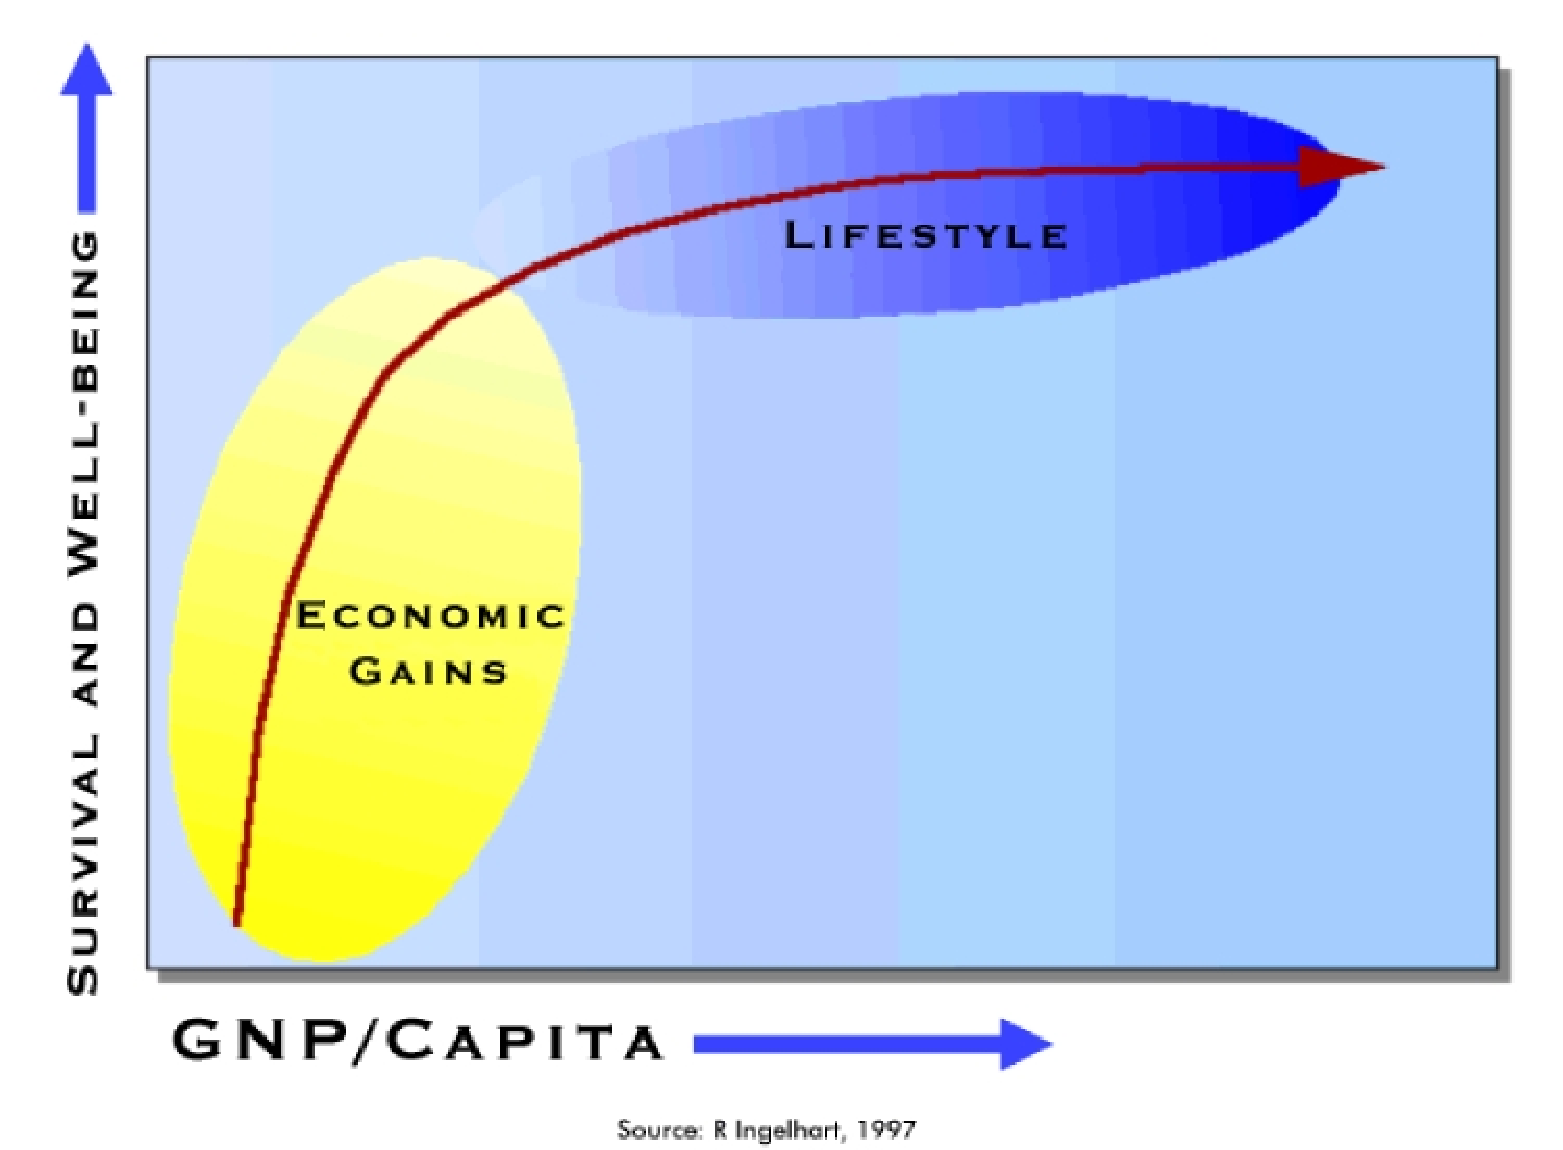
\includegraphics[height=2.5in]{/home/aok/papers/root/old/2011/eurostat_cities/tex/ingle.pdf}
%} 
 \caption{Well-being and income, \citep{inglehart97}.} \label{ingle}
  \end{centering}
\end{figure}


\subsection{Urbanicity Definition and results by different definition and
  sequentail elaboration}

we have 3 different operationalizatios of urbanicity: origianl 8 cat, collapse
one way and collapse the other way; and 3 sets of models: bivariate (iwth yr
dummies), esentially mean diff betwenn cat; basic set of controls;
necessary/important ones; full//extened (one in the body); and there is 4th one
over saturated but has most missing obs and hence postponed to the next section. 

where i dicuss controls in data and to literature where i slam
  burger and indeed as shown later comparing unadjusted means results in cities
   being happier notably due to confounding of higher income education and class


\begin{spacing}{.9} \begin{table}[H]\centering \caption{.} \label{d1} \begin{scriptsize} \begin{tabular}{p{1.8in}p{.5in}p{.5in}p{.5in}p{.5in}p{.5in}p{.5in}p{.5in}p{.5in}p{.5in}p{.5 in}p{.5in}p{.5 in}}\hline \input{../out/exT4-1.tex} \hline   * p$<$0.05, $+$ p$<$0.1; robust std err \end{tabular}\end{scriptsize}\caption{exT4-1}\end{table} \end{spacing}

\begin{spacing}{.9} \begin{table}[H]\centering \caption{.} \label{d1} \begin{scriptsize} \begin{tabular}{p{1.8in}p{.5in}p{.5in}p{.5in}p{.5in}p{.5in}p{.5in}p{.5in}p{.5in}p{.5in}p{.5 in}p{.5in}p{.5 in}}\hline \input{../out/exT3-1.tex} \hline   * p$<$0.05, $+$ p$<$0.1; robust std err \end{tabular}\end{scriptsize}\caption{exT3-1}\end{table} \end{spacing}

\begin{spacing}{.9} \begin{table}[H]\centering \caption{.} \label{d1} \begin{scriptsize} \begin{tabular}{p{1.8in}p{.5in}p{.5in}p{.5in}p{.5in}p{.5in}p{.5in}p{.5in}p{.5in}p{.5in}p{.5 in}p{.5in}p{.5 in}}\hline \input{../out/exT-1.tex} \hline   * p$<$0.05, $+$ p$<$0.1; robust std err \end{tabular}\end{scriptsize}\caption{exT-1}\end{table} \end{spacing}


\begin{spacing}{.9} \begin{table}[H]\centering \caption{.} \label{d1} \begin{scriptsize} \begin{tabular}{p{1.8in}p{.5in}p{.5in}p{.5in}p{.5in}p{.5in}p{.5in}p{.5in}p{.5in}p{.5in}p{.5 in}p{.5in}p{.5 in}}\hline \input{../out/exT4-2.tex} \hline   * p$<$0.05, $+$ p$<$0.1; robust std err \end{tabular}\end{scriptsize}\caption{exT4-2}\end{table} \end{spacing}

\begin{spacing}{.9} \begin{table}[H]\centering \caption{.} \label{d1} \begin{scriptsize} \begin{tabular}{p{1.8in}p{.5in}p{.5in}p{.5in}p{.5in}p{.5in}p{.5in}p{.5in}p{.5in}p{.5in}p{.5 in}p{.5in}p{.5 in}}\hline \input{../out/exT3-2.tex} \hline   * p$<$0.05, $+$ p$<$0.1; robust std err \end{tabular}\end{scriptsize}\caption{exT3-2}\end{table} \end{spacing}

\begin{spacing}{.9} \begin{table}[H]\centering \caption{.} \label{d1} \begin{scriptsize} \begin{tabular}{p{1.8in}p{.5in}p{.5in}p{.5in}p{.5in}p{.5in}p{.5in}p{.5in}p{.5in}p{.5in}p{.5 in}p{.5in}p{.5 in}}\hline \input{../out/exT-2.tex} \hline   * p$<$0.05, $+$ p$<$0.1; robust std err \end{tabular}\end{scriptsize}\caption{exT-2}\end{table} \end{spacing}


\begin{spacing}{.9} \begin{table}[H]\centering \caption{.} \label{d1} \begin{scriptsize} \begin{tabular}{p{1.8in}p{.5in}p{.5in}p{.5in}p{.5in}p{.5in}p{.5in}p{.5in}p{.5in}p{.5in}p{.5 in}p{.5in}p{.5 in}}\hline \input{../out/exT4-3.tex} \hline   * p$<$0.05, $+$ p$<$0.1; robust std err \end{tabular}\end{scriptsize}\caption{exT4-3}\end{table} \end{spacing}

\begin{spacing}{.9} \begin{table}[H]\centering \caption{.} \label{d1} \begin{scriptsize} \begin{tabular}{p{1.8in}p{.5in}p{.5in}p{.5in}p{.5in}p{.5in}p{.5in}p{.5in}p{.5in}p{.5in}p{.5 in}p{.5in}p{.5 in}}\hline \input{../out/exT3-3.tex} \hline   * p$<$0.05, $+$ p$<$0.1; robust std err \end{tabular}\end{scriptsize}\caption{exT3-3}\end{table} \end{spacing}

\begin{spacing}{.9} \begin{table}[H]\centering \caption{.} \label{d1} \begin{scriptsize} \begin{tabular}{p{1.8in}p{.5in}p{.5in}p{.5in}p{.5in}p{.5in}p{.5in}p{.5in}p{.5in}p{.5in}p{.5 in}p{.5in}p{.5 in}}\hline \input{../out/exT-3.tex} \hline   * p$<$0.05, $+$ p$<$0.1; robust std err \end{tabular}\end{scriptsize}\caption{exT-3}\end{table} \end{spacing}



\textbf{this one should be in appendix: 2 out of 10 again, but not rporting this
this is oversaturated and missing most countries}
\begin{spacing}{.9} \begin{table}[H]\centering \caption{.} \label{d1} \begin{scriptsize} \begin{tabular}{p{1.8in}p{.5in}p{.5in}p{.5in}p{.5in}p{.5in}p{.5in}p{.5in}p{.5in}p{.5in}p{.5 in}p{.5in}p{.5 in}}\hline \input{../out/exT3-4.tex} \hline   * p$<$0.05, $+$ p$<$0.1; robust std err \end{tabular}\end{scriptsize}\caption{exT3-4}\end{table} \end{spacing}



\textbf{so i think start with exT4-2 clean and easy and simple; then exT-3 to
  show detail and robustness}

\textbf{TODO meh yeah i guess drop this first table!!!}
note that all developed countres are less happy in cities, AUS (insiginifacnt
but sig in next table (\textbf{todo}check!)

\begin{spacing}{.9}
  \begin{table}[H]\centering \caption{.} \label{d1} \begin{scriptsize} \begin{tabular}{p{1.8in}p{.5in}p{.5in}p{.5in}p{.5in}p{.5in}p{.5in}p{.5in}p{.5in}p{.5in}p{.5
            in}p{.5in}p{.5 in}}\hline
        \input{../out/exT4-2.tex}
\hline  *** p$<$0.001, ** p$<$0.01, * p$<$0.05, $+$ p$<$0.1; robust std err
         \end{tabular}\end{scriptsize}\caption{exT4-2 OLS regressions of
         \texttt{swb} on \texttt{place size}, controls (not shown) are: enumerate}\end{table}
\end{spacing}

in atble \ref{exT4-2} several appear happier like BGD, IND, LTU, PAK, ROU, and
RUS, when adding more controls and full town cat that disappers except for 4 ctrioes


Results in table \ref{exT-3} are remarkable. In most countries large cities are less
happy than small settlements. Remarkably, without exception, in no developed
country city is happier than smallest areas. The only four countries where
people ar ehappier in large cities are: 

\begin{spacing}{.9}
  \begin{table}[H]\centering \caption{.} \label{d1} \begin{scriptsize} \begin{tabular}{p{1.8in}p{.5in}p{.5in}p{.5in}p{.5in}p{.5in}p{.5in}p{.5in}p{.5in}p{.5in}p{.5
            in}p{.5in}p{.5 in}}\hline
        \input{../out/exT-3.tex}
\hline  *** p$<$0.001, ** p$<$0.01, * p$<$0.05, $+$ p$<$0.1; robust std err
         \end{tabular}\end{scriptsize}\caption{exT-3; note robustness chech
         results are in SOM.}\end{table}
\end{spacing}
and tehre is even one more elaborate model\#4 in app with satfin and crime
like about \textbf{todo count lol} 20/70 neg of all and nly 4/18 of sig are pos
about 80 perc are neg :) or 5/21 in exT4-3

and the point is that the only ones that are sig and positive are wiers small
poor and most miserable countries except india which is a big puzzle

\textbf{TODO repreat it multiple times!} \textbf{TODO add NOR NLD}
so the conclusion is that in all develped countries AUS, CAN, DEU, ESP, ITA,
NZL, SWE, USA,  cities are less happy \footnote{at least in less elaborate
  specs, but even in most elaborate even if insig, still neg} in vast majority
of countries effect in ngeative, only positive in these 4:
russia, moldova and albania are all post soviet countries, they are likely to
still be very centralized where  power opportunity and resources are located in
large cities; india is clearly an outlier here and we dont have a good
explanation \texttt{[blind for peer review]} %\textbf{cite chourjua paper}



//----------------------------OLD




The limitation of \texttt{X049} is not only a low top bin for largest cities
(500k+), but also about a thrird of values missing. Future research can focus on
specific countries using other data or WVS data using \texttt{X049CS} variable,
which has country specific sizes of places, which however are not directly or
easily comparable--bins differ across countries and in some cases place is names
``major city'', ``Farm / Mountain / Fishing village,'' etc). 

show distributuion of place size by country!

\subsubsection{original 8 categories}
\subsubsection{0-5k v 500k+}
yeah this is following berry, but better have 0-5 so that more obs lol

\subsection{Crime and Cost of Living/financial satisfaction}
missing obs but here as a robustness check

TO WHERE I HAVE WE NEED TO CONTROL FOR CRIME:
Urban unhappiness is not only due
to urban problems such as crime and poverty.  Cities themselves, their core
defining characteristics, size and density, are related to unhappiness
\citep{aok_brfss_city_cize16}. 


yeh so one limitation is lack of crime; so bias on results cities wiuld be happier otherwhise

\begin{spacing}{.9} \begin{table}[H]\centering \caption{.} \label{d1} \begin{scriptsize} \begin{tabular}{p{1.8in}p{.5in}p{.5in}p{.5in}p{.5in}p{.5in}p{.5in}p{.5in}p{.5in}p{.5in}p{.5 in}p{.5in}p{.5 in}}\hline \input{../out/exT4-4.tex} \hline   * p$<$0.05, $+$ p$<$0.1; robust std err \end{tabular}\end{scriptsize}\caption{exT4-4}\end{table} \end{spacing}

\begin{spacing}{.9} \begin{table}[H]\centering \caption{.} \label{d1} \begin{scriptsize} \begin{tabular}{p{1.8in}p{.5in}p{.5in}p{.5in}p{.5in}p{.5in}p{.5in}p{.5in}p{.5in}p{.5in}p{.5 in}p{.5in}p{.5 in}}\hline \input{../out/exT3-4.tex} \hline   * p$<$0.05, $+$ p$<$0.1; robust std err \end{tabular}\end{scriptsize}\caption{exT3-4}\end{table} \end{spacing}

\begin{spacing}{.9} \begin{table}[H]\centering \caption{.} \label{d1} \begin{scriptsize} \begin{tabular}{p{1.8in}p{.5in}p{.5in}p{.5in}p{.5in}p{.5in}p{.5in}p{.5in}p{.5in}p{.5in}p{.5 in}p{.5in}p{.5 in}}\hline \input{../out/exT-4.tex} \hline   * p$<$0.05, $+$ p$<$0.1; robust std err \end{tabular}\end{scriptsize}\caption{exT-4}\end{table} \end{spacing}

\section{!!!PLAYING DROP THIS LATER}


\begin{spacing}{.9} \begin{table}[H]\centering \caption{.} \label{d1} \begin{scriptsize} \begin{tabular}{p{1.8in}p{.5in}p{.5in}p{.5in}p{.5in}p{.5in}p{.5in}p{.5in}p{.5in}p{.5in}p{.5 in}p{.5in}p{.5 in}}\hline \input{../out/ex1.tex} \hline   * p$<$0.05, $+$ p$<$0.1; robust std err \end{tabular}\end{scriptsize}\caption{ex1}\end{table} \end{spacing}

\begin{spacing}{.9} \begin{table}[H]\centering \caption{.} \label{d1} \begin{scriptsize} \begin{tabular}{p{1.8in}p{.5in}p{.5in}p{.5in}p{.5in}p{.5in}p{.5in}p{.5in}p{.5in}p{.5in}p{.5 in}p{.5in}p{.5 in}}\hline \input{../out/ex2.tex} \hline   * p$<$0.05, $+$ p$<$0.1; robust std err \end{tabular}\end{scriptsize}\caption{ex1}\end{table} \end{spacing}



\subsection{very first results}

Table \ref{a0} shows resuls of regression of \texttt{SWB} on place size dummies
(controlling for year dummies), which essentially differences in means for each
size category. Results are mixed, but large cities (500k-) and even medium sized
(100-500k) are often happier than the smallest category (the base case or
reference category, -2k). Usually diferences are small to moderate, about .5 (on
1-10 SWB scale), but sometimes large, larger than 1. Do mention the extremes and
think about why--but we do not have explanation for those. 

This is what the literature reports, tht results are mixed, in some cases cities
are happier, in some cases they are not. A key finding of this study is that
once we properly control for key predictors of SWB, almost uniformly large
cities (500k-) are less happy than the smallest settlements (-2k). Results are
shown in the body in table \ref{d1}.


%yah cannot use these 2--didnt drop properly these tiny categories so results
%dont make sense

% \begin{spacing}{.9}
%   \begin{table}[H]\centering \caption{.} \label{d1} \begin{scriptsize} \begin{tabular}{p{1.8in}p{.5in}p{.5in}p{.5in}p{.5in}p{.5in}p{.5in}p{.5in}p{.5in}p{.5in}p{.5
%             in}p{.5in}p{.5 in}}\hline
%         \input{/tmp/a0.tex}
% \hline  *** p$<$0.001, ** p$<$0.01, * p$<$0.05, $+$ p$<$0.1; robust std err
%          \end{tabular}\end{scriptsize}\caption{a0 OLS regressions of
%          \texttt{swb} on \texttt{place size}, controls (not shown) are: enumerate}\end{table}
% \end{spacing}

Results in table \ref{a} are remarkable. In most countries large cities are less
happy than small settlements. Remarkably, in no developed country city is
happier than smallest areas (with exception of KWT and SAU--these are
middle eastern and oil rich, where cities are glorious indeed)--and they are not
developed countries according to IMF or UN anyway neither have very high HDI.

% \begin{spacing}{.9}
%   \begin{table}[H]\centering \caption{.} \label{d1} \begin{scriptsize} \begin{tabular}{p{1.8in}p{.5in}p{.5in}p{.5in}p{.5in}p{.5in}p{.5in}p{.5in}p{.5in}p{.5in}p{.5
%             in}p{.5in}p{.5 in}}\hline
%         \input{/tmp/a.tex}
% \hline  *** p$<$0.001, ** p$<$0.01, * p$<$0.05, $+$ p$<$0.1; robust std err
%          \end{tabular}\end{scriptsize}\caption{a }\end{table}
% \end{spacing}


\end{spacing}
\end{document}
